% 05 --- Time Scales
\section{Time Scales in Molecular Simulation}

\begin{frame}{The Timestep $dt$ --- Heartbeat of MD}
	\begin{equation*}
		\mathbf{r}(t+dt) = \mathbf{r}(t)+\mathbf{v}dt+\tfrac12\mathbf{a}dt^2+\cdots
	\end{equation*}
	\begin{columns}[T,onlytextwidth]
		\column{0.5\textwidth}
		\begin{pitemize}
			\item $dt$ must resolve fastest vibration (bond $\sim10$ fs)
			\item Rule: $dt \lesssim 1$ fs (flexible), $2$ fs (constrained H)
			\item Too large \ensuremath{\rightarrow} \textbf{explosion} (energy drift)
		\end{pitemize}
		\column{0.5\textwidth}
		\begin{tikzpicture}[scale=1.0]
			\draw[->,accentcyan] (0,0)--(2.8,0) node[right]{$t$};
			\foreach \x in {0,0.5,1,1.5,2,2.5} {\fill[accentcyan] (\x,0) circle (2pt);}
			\draw[|<->|,neonyellow,thick] (0,-0.4) -- (0.5,-0.4) node[midway,below,color=neonyellow]{$dt$};
			\only<2>{\node[draw=neonpink,fill=neonpink!15,rounded corners=1mm,inner sep=1mm,text=bgblack] at (1.4,1) {SHAKE \ensuremath{\rightarrow} $dt=2$ fs!};}
		\end{tikzpicture}
	\end{columns}
\end{frame}

\begin{frame}{Hierarchy of Time}
	\begin{center}
		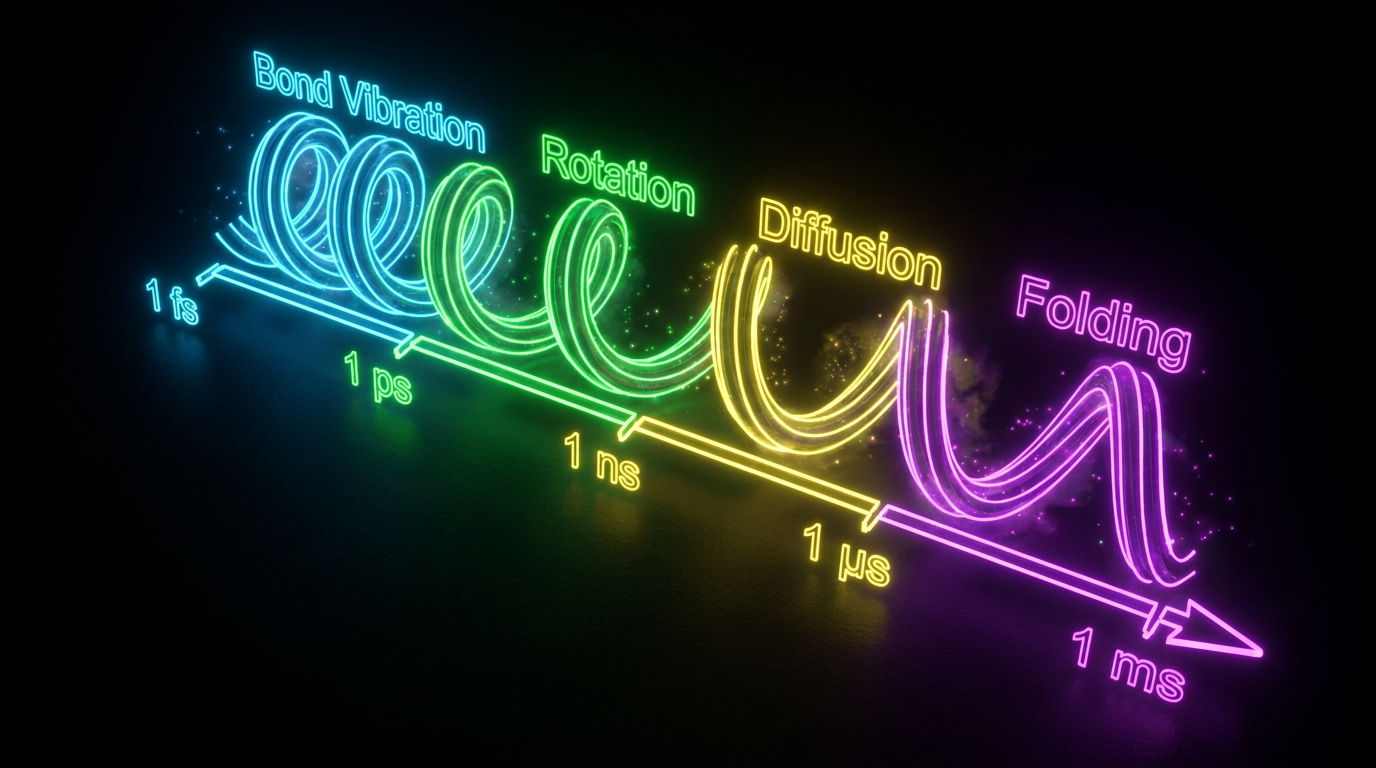
\includegraphics[width=0.85\linewidth]{assets/figures/timescale_hierarchy.png}
	\end{center}
	\begin{pitemize}
		\item \textbf{fs} \ensuremath{\rightarrow} bonds, \textbf{ps} \ensuremath{\rightarrow} water, \textbf{ns} \ensuremath{\rightarrow} sidechains, \textbf{$\mu$s} \ensuremath{\rightarrow} folding, \textbf{ms--s} \ensuremath{\rightarrow} rare
	\end{pitemize}
\end{frame}

\begin{frame}{Simulation Length --- $T = N_{\text{steps}}\times dt$}
	\begin{columns}[T,onlytextwidth]
		\column{0.5\textwidth}
		\begin{pitemize}
			\item $N_{\text{steps}} = T/dt$
			\item $100$ ns at $2$ fs \ensuremath{\rightarrow} $50$M steps
			\item Cost: $10^9$ force calls = GPU-days
		\end{pitemize}
		\column{0.5\textwidth}
		\begin{tikzpicture}[scale=1.0]
			\draw[accentcyan,thick] (0,0) rectangle (2.6,1.4);
			\foreach \y in {0.2,0.5,0.8,1.1} {\draw[softgray] (0,\y) -- (2.6,\y);}
			\node[color=fgwhite] at (1.3,1.2) {steps};
			\draw[->,thick,neonyellow] (0,-0.3) -- (2.6,-0.3) node[midway,below]{$T$};
			\draw[|<->|,accentcyan,thick] (0,1.6) -- (0.4,1.6) node[midway,above]{$dt$};
		\end{tikzpicture}
	\end{columns}
\end{frame}

\begin{frame}{Meme --- Timescales (This is Fine + Race)}
	\begin{columns}[T,onlytextwidth]
		\column{0.5\textwidth}
		\memeinclude[width=\linewidth]{assets/memes/thisisfine_meme.png}
		{\footnotesize\color{softgray} This is Fine: dt=5 fs in production}
		\column{0.5\textwidth}
		\memeinclude[width=\linewidth]{assets/memes/timescales_meme.png}
		{\footnotesize\color{softgray} Snail (ms) vs Cheetah (fs)}
	\end{columns}
\end{frame}

\begin{frame}{Interpretation --- Timescales}
	\interpret{
		\textbf{$dt$} · 1--2 fs · \textbf{hierarchy} · fs\ensuremath{\rightarrow}ms · \textbf{$T=Ndt$} · steps = cost · \textbf{rare} · need tricks · \textbf{clock} vs \textbf{biology} mismatch
	}
\end{frame}
